\begin{figure}[h]
	\centering
	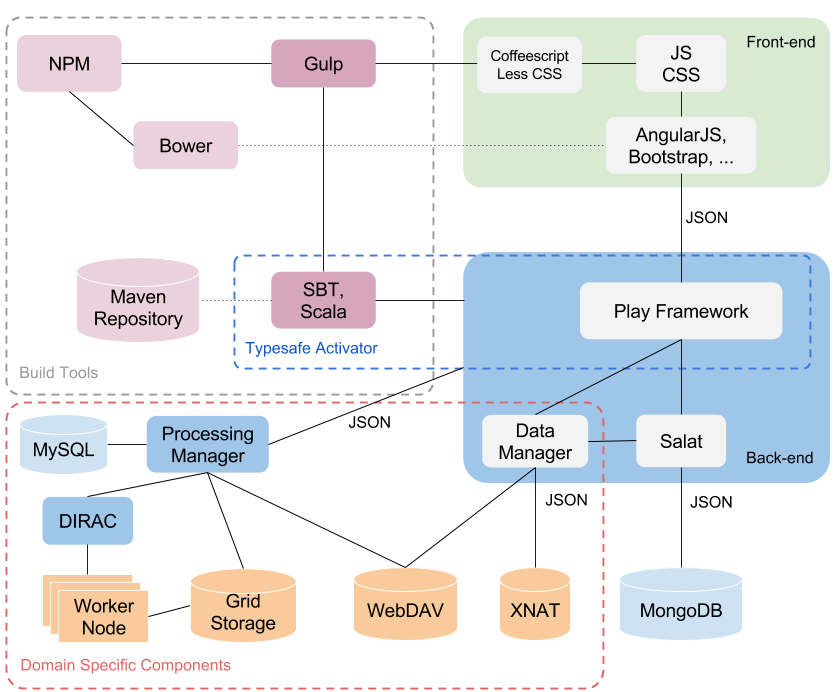
\includegraphics[width=0.7\linewidth]{images/rosemary-architecture}
	\caption{
		Rosemary architecture including domain specific components (denoted with red dashed border).
		It describes the implementation of the \nsg{} back-end and front-end, together with the specific build tools used during development.
	}
	\label{fig:reuse-rosemary-architecture}
\end{figure}

\paragraph{Rosemary: Architecture}
The overall workings of Rosemary have been described in the previous section.
Below the architecture and data model will be explained before going into details of the \ivfprototype{} implementation, which will be described in section \ref{implementation}.

The Rosemary architecture is shown in figure \ref{fig:reuse-rosemary-architecture}.
It depicts: the back-end, the front-end, \nsg{} specific components, and development build tools.
For the back-end the Play Framework \cite{play} is used.
It is written with the Scala \cite{scala} programming language which is interoperable with Java.
As a database mongoDB \cite{mongo} is used, a document-oriented database.
Communication between the back-end and the database is done with JSON \cite{json} and the Scala library `Salat' is used to serialise the JSON information into Scala classes.
The back-end exposes a RESTful API which can be accessed by the front-end.

The front-end is based on the AngularJS \cite{angular} framework and coded with Coffeescript \cite{coffeescript}, which is compiled into JavaScript.
For layout and styling HTML and Less \cite{less} are used, Less compiles into Cascading Style Sheets (CSS).
To provide a pleasant user experience the front-end is developed as a web application. 
Data is loaded asynchronous through the RESTful API and stored at the client's side to give the feel of a native application.

\paragraph{Rosemary: data model}
The yellow components in figure \ref{fig:implementation-rosemary-dm} depict the Rosemary data model with the neuroscience specific items removed, the unedited data model can be found in appendix \ref{unedited-datamodel}.
The model contains six main data objects: {\tt Datum}, {\tt Tag}, {\tt Rights}, {\tt User}, {\tt Notification}, and {\tt Thread}.
The {\tt Tag}, {\tt Notification}, and {\tt Rights} objects are inherited to describe a specific instance; for example, {\tt WorkspaceTag} is a kind of {\tt Tag}.

A short description of the main objects will be given for better understanding of the model.
A {\tt Datum} is a single piece of data and its metadata. 
For the Rosemary a {\tt Datum} might be a reference to an MRI image and metadata about the scanned patient.
{\tt Datum}s may be tagged with the {\tt Tag} object. 
For example, the {\tt UserTag} is a tag defined by the user and attached to a set of {\tt Datum}s for identification.
{\tt Tag}s are also used to manage access rights: each {\tt Tag} has a specific {\tt Rights} attached to it.
A {\tt Rights} object in its turn contains a set of {\tt User}s which have access to the tagged data, for example a {\tt UserTag} (and the associated data) may be shared among users by adding them as members in the tag's rights.
The {\tt Notification} object stores data about process milestones which can be displayed in the user interface, for example, when a message is sent by another user or the system.
Lastly, the {\tt Thread} keeps track of messages send back and forth in conversations.

The data model and its implementation provide some interesting possibilities.
For example, a {\tt Datum} can be tracked and reused endlessly by applying a {\tt Tag} object.
One possible usage of this is implementation of access control, which can be applied by tagging a {\tt Datum} with a {\tt WorkspaceTag} that is owned by a {\tt User}.
Many different constructs of this sort can be achieved without ever touching the structure of the  original Rosemary model itself.

\begin{figure}[h]
	\centering
	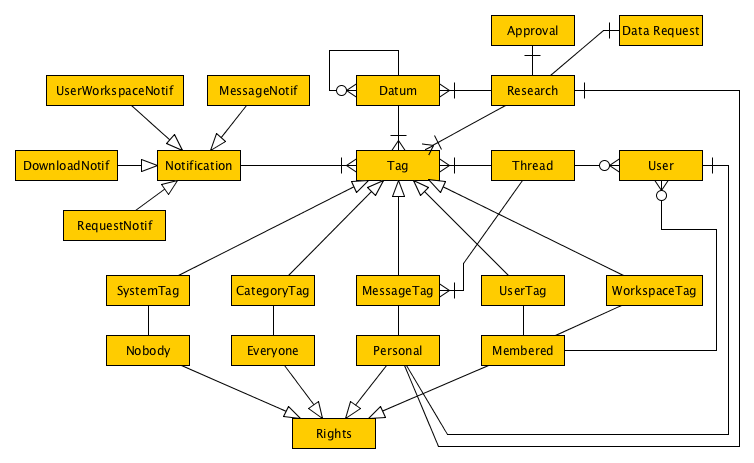
\includegraphics[width=0.8\linewidth]{images/datamodel-adapted}
	\caption{
		Rosemary data model as implemented.
		Differences between the implemented \ivfprototype{} model and the original Rosemary model are shown in blue.
		Note that \nsg{} specific data objects are omitted as they are not used in the \ivfprototype{} implementation.
		Describes workspace, tagging, datum, notification, and research models.
		The unedited data model can be found in appendix \ref{unedited-datamodel}.
	}
	\label{fig:implementation-rosemary-dm}
\end{figure}